\documentclass{article}
%%%%%%%%%%%%%%%%%%%%%%%%%%%%%%%%%%%
\title{ME760 Homework 3}
\author{John Boyington}
\date{November 3, 2017}

% Optional disclaimer: remove this command to hide
%\disclaimer{Notice: This manuscript is a work of fiction. Any resemblance to
%actual articles, living or dead, is purely coincidental.}

%%%% packages and definitions (optional)
\usepackage{graphicx} % allows inclusion of graphics
\usepackage{microtype} % improves typography for PDF
\usepackage{xcolor}
\usepackage{amsmath}
\usepackage{amssymb}
\usepackage{amsthm}
\usepackage[amssymb,cdot]{SIunits}
\usepackage{bm}
\usepackage{enumitem}
\usepackage[margin=0.75in]{geometry}
\usepackage{mathrsfs}
\usepackage{tabulary}
\usepackage{booktabs}
\usepackage{listings}
\usepackage{minibox}
\lstset{basicstyle=\ttfamily,
  showstringspaces=false,
  commentstyle=\color{red},
  keywordstyle=\color{blue},
  numbers=left
}

\renewcommand{\baselinestretch}{1.3}
\newcommand{\SN}{S$_N$}
\renewcommand{\vec}[1]{\bm{#1}} %vector is bold italic
\newcommand{\vd}{\bm{\cdot}} % slightly bold vector dot
\newcommand{\grad}{\vec{\nabla}} % gradient
\newcommand{\ud}{\mathop{}\!\mathrm{d}} % upright derivative symbol
\providecommand{\e}[1]{\ensuremath{\vd 10^{#1}}}
\newcommand{\oper}[1]{\mathcal{#1}}
\newcommand{\EQ}[1]{Eq.~(\ref{#1})}               %-- Eq. (refeq)
\newcommand{\EQUATION}[1]{Equation~(\ref{#1})}    %-- Equation (refeq)
\newcommand{\FIG}[1]{Fig.~\ref{#1}}               %-- Fig. refig
\newcommand{\FIGURE}[1]{\FIG{#1}}          %-- Figure refig
\newcommand{\TAB}[1]{Table~\ref{#1}}              %-- Table tablref
\newcommand{\EQS}[2]{Eqs.~(\ref{#1})--(\ref{#2})}            %-- Eqs. (refeqs)
\newcommand{\EQUATIONS}[2]{Equations~(\ref{#1})--(\ref{#2})} %-- Eqs. (refeqs)
\newcommand{\EQSTWO}[2]{Eqs.~(\ref{#1})~and~(\ref{#2})} %-- Eqs. (refeqs)
\newcommand{\EQUATIONSTWO}[2]{Equations~(\ref{#1})~and~(\ref{#2})}             
%-- Eqs. (refeqs
\newcommand{\BOXEQ}[1]{\mbox{\fboxsep=.13in $$
        \framebox{#1} $$ } }    %-- box around equation
\newcommand{\SEC}[1]{Section~\ref{#1}}               %-- Eq. (refeq)
\newcommand{\REF}[1]{Ref.~\citen{#1}}               %-- Eq. (refeq)
\DeclareMathOperator*{\dotp}{{\scriptscriptstyle \stackrel{\bullet}{{}}}}

\begin{document}
    \maketitle
    
    %%%%%%%%%%%%%%%%%%%%%%%%%%%%%%%%%%%%%%%%%%%%%%%%%%%%%%%%%%%%%%%%%%%%
    %                           problem 1
    %%%%%%%%%%%%%%%%%%%%%%%%%%%%%%%%%%%%%%%%%%%%%%%%%%%%%%%%%%%%%%%%%%%%
    
    \section*{Problem 1}
    \subsection*{Problem Statement}
    Estimate the spectral radius of the following matrix. Show your work.
    
        \[{\bf A} =\begin{bmatrix}
    		7&0&3\\
    		2&1&1\\
    		2&0&2\\
    	\end{bmatrix}\]
    
    \subsection*{Solution}
    Find the determinate of {\bf B} if {\bf B} is {\bf A $-$ I$\lambda$} to obtain eigenvalues. \\
    
    \begin{centering}
    
    $(7 - \lambda)[(1 - \lambda)(2 - \lambda)] + 3[-2(1 - \lambda)] = 0$ \\
    
    $(7 - \lambda)[(1 - \lambda)(2 - \lambda)]  -6(1 - \lambda) = 0$ \\
    
    $(1 - \lambda)[(7 - \lambda)(2 - \lambda) - 6] = 0$ \\
    
    $\lambda = 1,$ \\
    
    $14 - 9\lambda + \lambda^{2} - 6 = 0$ \\
    
    $8 - 9\lambda + \lambda^{2} = 0$ \\
    
    $(\lambda - 8)(\lambda - 1) = 0$ \\
    
    $\lambda = 8, 1, 1$ \\
    
    \end{centering}
    
    The spectral radius, $\rho$, is the largest eigenvalue of the matrix.
    
    \begin{centering}
    
    \fbox{$\rho(${\bf A}$) = 8$}
    
    \end{centering}
    
    \pagebreak
     
    %%%%%%%%%%%%%%%%%%%%%%%%%%%%%%%%%%%%%%%%%%%%%%%%%%%%%%%%%%%%%%%%%%%%
    %                           problem 2
    %%%%%%%%%%%%%%%%%%%%%%%%%%%%%%%%%%%%%%%%%%%%%%%%%%%%%%%%%%%%%%%%%%%%
    
    \section*{Problem 2}
    \subsection*{Problem Statement}
    
    Given the curve C: {\bf r}$(u) = ${\bf i}$ \cos u + ${\bf j}$ 2 \sin u$, find (a) a tangent vector {\bf r}$' (u)$ and the corresponding unit vector $\mathbf{\hat{r}'}(u)$, (b) {\bf r}$'$ and $\mathbf{\hat{r}'}$ at the point $P$ : (1/2, $\sqrt{3}$, 0), and (c) the equation of the line through $P$ that is tangent to the curve. Sketch the curve and the tangent.
    
    
    \subsection*{Solution}
    \begin{centering}
    (a) \\
    \fbox{$\mathbf{r'}(u) = \hat{i} (-\sin{u}) + \hat{j}(2 \cos{u})$} \\
    $\mathbf{\hat{r}'}(u) = \frac{1}{\sqrt{\sin ^2 u + 2 \cos ^2 u}} \mathbf{r'}(u)$ \\
    \fbox{$\mathbf{\hat{r}'}(u) = \frac{1}{\sqrt{3}}[ \hat{i} (-\sin{u}) + \hat{j}(2 \cos{u})]$} \\
    (b) \\
    at $P(1/2, \sqrt{3}, 0), u = \pi/3$ \\
    \fbox{$\mathbf{r'}(\frac{\pi}{3}) = -\frac{\sqrt{3}}{2}\hat{i} + 1 \hat{j}$} \\
    \fbox{$\mathbf{\hat{r}'}(\frac{\pi}{3}) = -\frac{1}{2}\hat{i} + \frac{1}{\sqrt{3}} \hat{j}$} \\
    (c) \\
    $l = \mathbf{\vec{P}} + \lambda \mathbf{\hat{r}'}$ \\
    $l = \frac{1}{2} (1 - \lambda) \hat{i} + \sqrt{3} (1 + \frac{1}{3} \lambda) \ hat{j}$ \\
    \fbox{$l = \frac{1}{2} (1 - \lambda) \hat{i} + \sqrt{3} (1 + \frac{1}{3} \lambda) \hat{j}$} \\
    
    \begin{figure}[h]
    	\centering
    	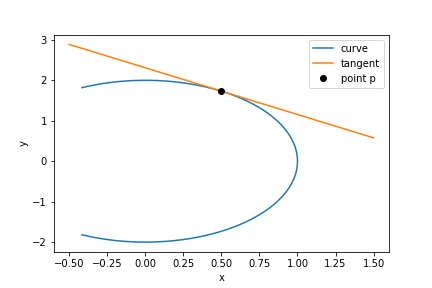
\includegraphics[height=0.4\textheight]{p2}
    \end{figure}
    
    
    
    \end{centering}
    
    \pagebreak
    
    %%%%%%%%%%%%%%%%%%%%%%%%%%%%%%%%%%%%%%%%%%%%%%%%%%%%%%%%%%%%%%%%%%%%
    %                           problem 3
    %%%%%%%%%%%%%%%%%%%%%%%%%%%%%%%%%%%%%%%%%%%%%%%%%%%%%%%%%%%%%%%%%%%%
    
    \section*{Problem 3}
    \subsection*{Problem Statement}
    Find the length of the circular helix $\mathbf{r}(u) = \mathbf{i} a \cos u + \mathbf{j} a \sin u + \mathbf{k}cu$ from $(a, 0, 0)$ to $(a, 0, 2\pi c)$.
    
    
    \subsection*{Solution}
    
    \begin{centering}
    
    $s = \int_a^b |\mathbf{r'}(u)| du = \int_a^b \sqrt{\mathbf{r'}(u) \cdot \mathbf{r'}(u)}$ \\
    $s = \int_0^{2\pi} \sqrt{a^2 \sin ^2 u + a^2 \cos^2 u + c^2} du$ \\
    $s = \int_0^{2\pi} \sqrt{a^2 + c^2} du$ \\
    $s = \sqrt{a^2 + c^2} u |_0^{2\pi}$ \\
    \fbox{$s = 2 \pi \sqrt{a^2 + c^2}$} \\

	\end{centering}
    
    \pagebreak
    
    %%%%%%%%%%%%%%%%%%%%%%%%%%%%%%%%%%%%%%%%%%%%%%%%%%%%%%%%%%%%%%%%%%%%
    %                           problem 4
    %%%%%%%%%%%%%%%%%%%%%%%%%%%%%%%%%%%%%%%%%%%%%%%%%%%%%%%%%%%%%%%%%%%%
    
    \section*{Problem 4}
    \subsection*{Problem Statement}
    
    Sketch $\mathbf{r}(t) = \mathbf{i}(R \sin \omega t + ω\omega Rt) + \mathbf{j}(R cos \omega t + R)$ taking $R = 1$ and $\omega = 1$. This curve is called a cycloid and is the path of a point on the rim of a wheel of radius R that rolls without slipping along the $x$-axis. Find the velocity {\bf v} and the acceleration {\bf a} at the maximum and minimum $y$-values of the curve.
    
    
    \subsection*{Solution}
    
    \begin{centering}
    
    \begin{figure}[h]
    	\centering
    	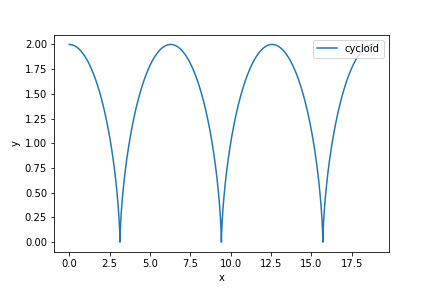
\includegraphics[height=0.4\textheight]{cycloid}
    \end{figure}
    
    
    $R = \omega = 1$ \\
    $\mathbf{r}(t) = \mathbf{i}(\sin{t} + t) + \mathbf{j}(\cos{t} + 1)$ \\
    $\mathbf{v}(t) = \frac{dr}{dt}$ \\
    $\mathbf{v}(t) = \mathbf{i}(\cos{t} + t) - \mathbf{j}(\sin{t})$ \\
    $\mathbf{a}(t) = \frac{dv}{dt}$ \\
    $\mathbf{a}(t) = - \mathbf{i}(\sin{t}) - \mathbf{j}(\sin{t})$ \\
    \minibox[frame]{max: $t = 0, x = 0, y = 2$ \\
    $\mathbf{v}(t) = 2 \mathbf{i}$ \\
    $\mathbf{a}(t) = -1 \mathbf{j}$ \\
    min: $t = 0\pi, x = \pi, y = 0$ \\
    $\mathbf{v}(t) = 0$ \\
    $\mathbf{a}(t) = 1 \mathbf{j}$} \\
    
    
    
    \end{centering}
    
    
    
    \pagebreak
    
    %%%%%%%%%%%%%%%%%%%%%%%%%%%%%%%%%%%%%%%%%%%%%%%%%%%%%%%%%%%%%%%%%%%%
    %                           problem 5
    %%%%%%%%%%%%%%%%%%%%%%%%%%%%%%%%%%%%%%%%%%%%%%%%%%%%%%%%%%%%%%%%%%%%
    
    \section*{Problem 5}
    \subsection*{Problem Statement}
    The flow of heat in a temperature field takes place in the direction of the maximum decrease of temperature. For the temperature field $T (x, y, z) = z/(x^2 + y^2)$ find this direction in general and at the point $(0, 1, 2)$.
    
    
    \subsection*{Solution}
    
    \begin{centering}
    
    Find $\grad T(x, y, z)$ \\
    $\frac{\partial T}{\partial x} = \frac{-2xz}{(x^2 + y^2)^2} \mathbf{i}$ \\
    $\frac{\partial T}{\partial y} = \frac{-2yz}{(x^2 + y^2)^2} \mathbf{j}$ \\
    $\frac{\partial T}{\partial z} = \frac{1}{(x^2 + y^2)^2} \mathbf{k}$ \\
    \fbox{$\grad T(x, y, z) = \frac{-2xz}{(x^2 + y^2)^2} \mathbf{i} - \frac{2yz}{(x^2 + y^2)^2} \mathbf{j} + \frac{1}{(x^2 + y^2)^2} \mathbf{k}$} \\
    At $P(0, 1, 2)$: \\
    $0\mathbf{i} - \frac{2(1)(2)}{1} \mathbf{j} + 1 \mathbf{k}$ \\
    \fbox{ $-4 \mathbf{j} + \mathbf{k}$} \\
    
    
    \end{centering}
    \pagebreak
    
    %%%%%%%%%%%%%%%%%%%%%%%%%%%%%%%%%%%%%%%%%%%%%%%%%%%%%%%%%%%%%%%%%%%%
    %                           problem 6
    %%%%%%%%%%%%%%%%%%%%%%%%%%%%%%%%%%%%%%%%%%%%%%%%%%%%%%%%%%%%%%%%%%%%
    
    \section*{Problem 6}
    \subsection*{Problem Statement}
    
    Find the unit normal (a) to the surface $ax + by + cz + d = 0$ at any point $P$, and (b) to the surface $x^2 + y^2 + z^2 = 26$ at the point $(1, 4, 3)$.
    
    
    \subsection*{Solution}
    
    \begin{centering}
    
    (a) \\
    \fbox{$\hat{n} = \frac{\grad f(\mathbf{r})}{|\grad f(\mathbf{r})|} = \frac{a\mathbf{i} + b\mathbf{j} + c\mathbf{k}}{\sqrt{a^2 + b^2 + c^2}}$} \\
    (b) \\
    $\grad  f(\mathbf{r}) = 2x \mathbf{i} + 2y \mathbf{j} + 2z \mathbf{k}$ \\
    At point $P$: \\
    $ = 2 \mathbf{i} + 8 \mathbf{j} + 6 \mathbf{k}$ \\
    magnitude $= \sqrt{2^2 + 8^2 + 6^2} = \sqrt{104} = 2\sqrt{26}$ \\
    \fbox{$\hat{n} = \frac{1}{\sqrt{26}}(1 \mathbf{i} + 4 \mathbf{j} + 3 \mathbf{k})$} \\
    
    
    \end{centering}
    
    
    
    
    \pagebreak
    
    %%%%%%%%%%%%%%%%%%%%%%%%%%%%%%%%%%%%%%%%%%%%%%%%%%%%%%%%%%%%%%%%%%%%
    %                           problem 7
    %%%%%%%%%%%%%%%%%%%%%%%%%%%%%%%%%%%%%%%%%%%%%%%%%%%%%%%%%%%%%%%%%%%%
    
    \section*{Problem 7}
    \subsection*{Problem Statement}
    Find the divergence of $(-\mathbf{i}y + \mathbf{j}x)/(x^2 + y^2)$.
    
    
    \subsection*{Solution}
    
    \begin{centering}
    
    $\grad \cdot \mathbf{v} = \frac{\partial V_x}{\partial x} + \frac{\partial V_y}{\partial y} + \frac{\partial V_y}{\partial y}$ \\
    $\mathbf{v} = \frac{-y}{x^2 + y^2}\mathbf{i} + \frac{x}{x^2 + y^2}\mathbf{j}$ \\
    Apply the quotient rule for derivatives. \\
    $\grad \cdot \mathbf{v} = \frac{2xy}{(x^2 + y^2)^2} - \frac{2xy}{(x^2 + y^2)^2}$ \\
    \fbox{$\grad \cdot \mathbf{v} = 0$} \\
    
    
    
    \end{centering}
    
    \pagebreak
    %%%%%%%%%%%%%%%%%%%%%%%%%%%%%%%%%%%%%%%%%%%%%%%%%%%%%%%%%%%%%%%%%%%%
    %                           problem 8
    %%%%%%%%%%%%%%%%%%%%%%%%%%%%%%%%%%%%%%%%%%%%%%%%%%%%%%%%%%%%%%%%%%%%
    
    \section*{Problem 8}
    \subsection*{Problem Statement}
    Prove that $\grad \cdot ( \grad \times ${\bf v}$) = 0$.
    
    
    \subsection*{Solution}
    
    \begin{centering}
    
    {\bf v} $= u\hat{i} + v\hat{j} + w\hat{k}$
    
    $\grad \times ${\bf v}$ =  \begin{bmatrix}
                                \hat{i}&\hat{j}&\hat{k}\\
                                \frac{\partial}{\partial x}
                                & \frac{\partial}{\partial y}
                                & \frac{\partial}{\partial z}\\
                                u&v&w\\
                                \end{bmatrix}$
     
     $\grad \times ${\bf v}
     $= \hat{i}(\frac{\partial}{\partial y} w - \frac{\partial}{\partial z} v)
      + \hat{j}(\frac{\partial}{\partial z} u - \frac{\partial}{\partial x} w)
      + \hat{k}(\frac{\partial}{\partial x} v - \frac{\partial}{\partial y} u)$ \\
      
      Then do $div$ of that quantity.
    
    
      $ 0
      = (\frac{\partial^2}{\partial x \partial y} w - \frac{\partial^2}{\partial x \partial z} v)
      + (\frac{\partial^2}{\partial y \partial z} u - \frac{\partial^2}{\partial y \partial x} w)
      + (\frac{\partial^2}{\partial x \partial z} v - \frac{\partial^2}{\partial y \partial z} u)$ \\
    
    Each term in the equation above will cancel out.
    
    \end{centering}
    
\end{document}